%\RequirePackage{atbegshi}
\documentclass{beamer}

\usetheme{Rochester}
\usepackage{amssymb}
%\usepackage[cmex10]{amsmath}
\usepackage{stmaryrd,epsfig,psfrag}
\usepackage[english]{babel}
\usepackage{tikz,pgf,pgfplots}
\pgfplotsset{compat=newest}
\usepgflibrary{shapes}
\usetikzlibrary{%
  arrows,%
  mindmap,%mindmap
  calendar,%calendar
  decorations,%decorations
  snakes,%snakes
  shapes.misc,% wg. rounded rectangle
  shapes.arrows,%
	shapes.callouts, %
  shapes,%
  chains,%
  matrix,%
  positioning,% wg. " of "
  scopes,%
  decorations.pathmorphing,% /pgf/decoration/random steps | erste Graphik
	decorations.text, %
  shadows,%
  backgrounds,%
  fit,%
  petri%
}

% Radius of regular polygons
\newdimen\R
\R=0.8cm

\definecolor{tutorial}{RGB}{50,93,61}


\title{Machine Learning for Anomaly Detection in Overlapping Aerial Image Streams}
\author{Travis Taghavi}
\institute{Electrical and Computer Engineering \\ Texas A\&M University}

%\setbeamertemplate{footline}[page number]
\setbeamertemplate{navigation symbols}{\textcolor{black}{\insertframenumber / \inserttotalframenumber}}

\begin{document}

\begin{frame}
  \titlepage
\end{frame}


\begin{frame}
\frametitle{Outline}
\begin{itemize}
  \item \textbf{Introduction}
  \item\vspace{0.5cm} Problem Setting
  \item\vspace{0.5cm} Image Features
  \item \vspace{0.5cm}Learning Models
  \item \vspace{0.5cm} Results
  \item \vspace{0.5cm}Conclusions
\end{itemize}
\end{frame}


\begin{frame}
\frametitle{Acknowledgments}
This material is based, in part, upon work supported by the TEES-AgriLife Center for Bioinformatics and Genomic Systems Engineering (CBGSE). Any opinion, findings, and conclusions or recommendations expressed in this material are those of the authors and do not necessarily reflect the views of the CBGSE.
\end{frame}


\begin{frame}
\frametitle{Motivation}
\begin{columns}
  \column{.43\textwidth}
    \begin{itemize}
      \item Water and resource scarcity present a unique and impending challenge in agriculture
      \item Precision agriculture provides promising avenue to alleviate related issues
      \item Aerial imaging of plots is a vital step in precision agriculture, though challenges remain
    \end{itemize}
  \column{.55\textwidth}
  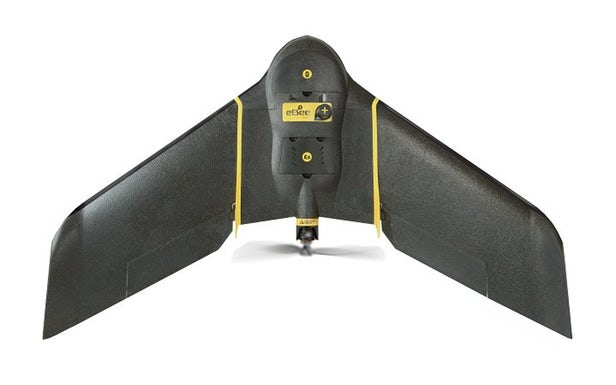
\includegraphics[width = 5cm]{Figures/ebee}
\end{columns}
\end{frame}


\begin{frame}
\frametitle{Unmanned Aerial Systems (UAS)}
\begin{columns}
  \column{0.48\textwidth}
    \begin{center}
      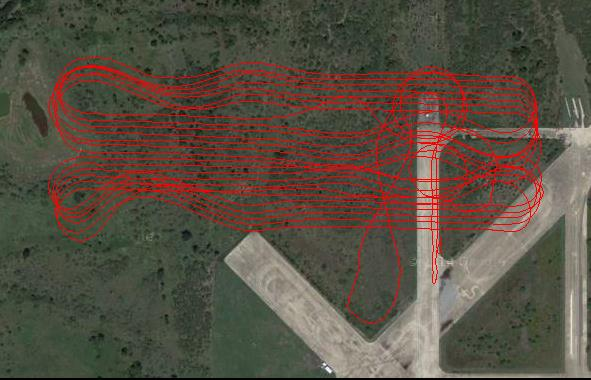
\includegraphics[width=5cm]{Figures/flightpath}
    \end{center}
  \column{0.49\textwidth}
    \begin{itemize}
      \item Fixed or rotary wing aircraft that are flown remotely - either manually or automatically
      \item Imaging system fixed to the bottom, pointed directly towards the ground
      \item Take images over a flight-path which is generated to cover area of interest
      \item Images are stitched together in post to create single map
    \end{itemize}
\end{columns}
\end{frame}


\begin{frame}
\frametitle{Image Mosaicking}
\begin{itemize}
  \item The process of stitching together a series of images into a single image
  \begin{itemize}
    \item Simple example: panoramic picture
  \end{itemize}
  \item Complex programs such as Pix4D and OpenDroneMap perform this in post, generally on a specialized processing computer
  \item Utilizes GPS coordinates and calculations on image features to determine where to stitch images
  \item For optimal performance, requirements on image scale and necessary overlap between images
  \item Final output useful for obtaining statistics on crops, locations of invasive species, under/over-hydrated areas, etc.
\end{itemize}
\end{frame}


\begin{frame}
\frametitle{Outline}
\begin{itemize}
  \item Introduction
  \item\vspace{0.5cm} \textbf{Problem Setting}
  \item\vspace{0.5cm} Image Features
  \item \vspace{0.5cm}Learning Models
  \item \vspace{0.5cm} Results
  \item \vspace{0.5cm}Conclusions
\end{itemize}
\end{frame}


\begin{frame}
\frametitle{Data Pipeline}
\begin{itemize}
  \item Flights planned by members of TAMU GEOSAT, based on needs of agricultural researchers
  \item Flight height/speed, as well as image frequency, determined to obtain approximately 75\% overlap between images
  \item After a flight is completed, the raw images transferred to network drive, cleaned and preprocessed
  \item Images then passed to a mosaicking program where they are processed for a few hours up to a few days
  \item Final mosaic and raw images returned to researchers
\end{itemize}
\end{frame}


\begin{frame}
\frametitle{Problem Formulation}
\begin{itemize}
  \item Due to inconsistencies inherent in almost all flight, the UAS may experience tilting or swinging without warning
  \item Results in images which are not pointed directly towards the ground, do not contain the required overlap - anomalous images
  \item Anomalous images irreconcilable to the mosaicking program, cause longer processing times and sub-optimal output
  \item Goal is to create a system to quickly identify these images 
  \begin{itemize}
    \item Either run as preprocessing step to remove, or during imaging so the images can be flagged and retaken if necessary
  \end{itemize}
\end{itemize}
\end{frame}

\begin{frame}
\frametitle{Acceptable Image Stream}
\begin{columns}
\column{0.001\textwidth}
\column{0.999\textwidth}
\begin{centering}
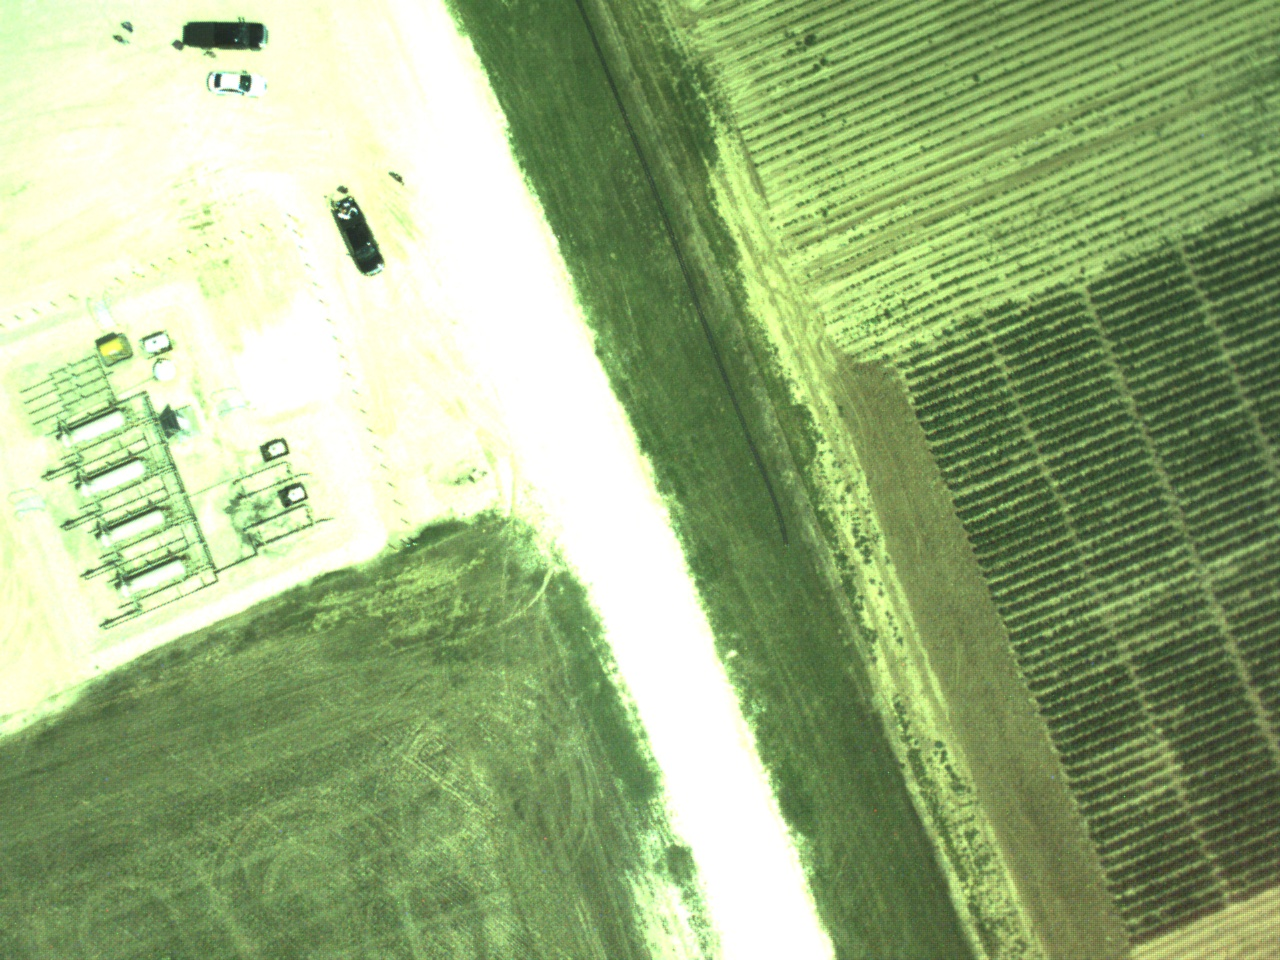
\includegraphics[width = 10cm]{Figures/good1}
\end{centering}
\end{columns}
\end{frame}


\begin{frame} [noframenumbering]
\frametitle{Acceptable Image Stream}
\begin{columns}
\column{0.001\textwidth}
\column{0.999\textwidth}
\begin{centering}
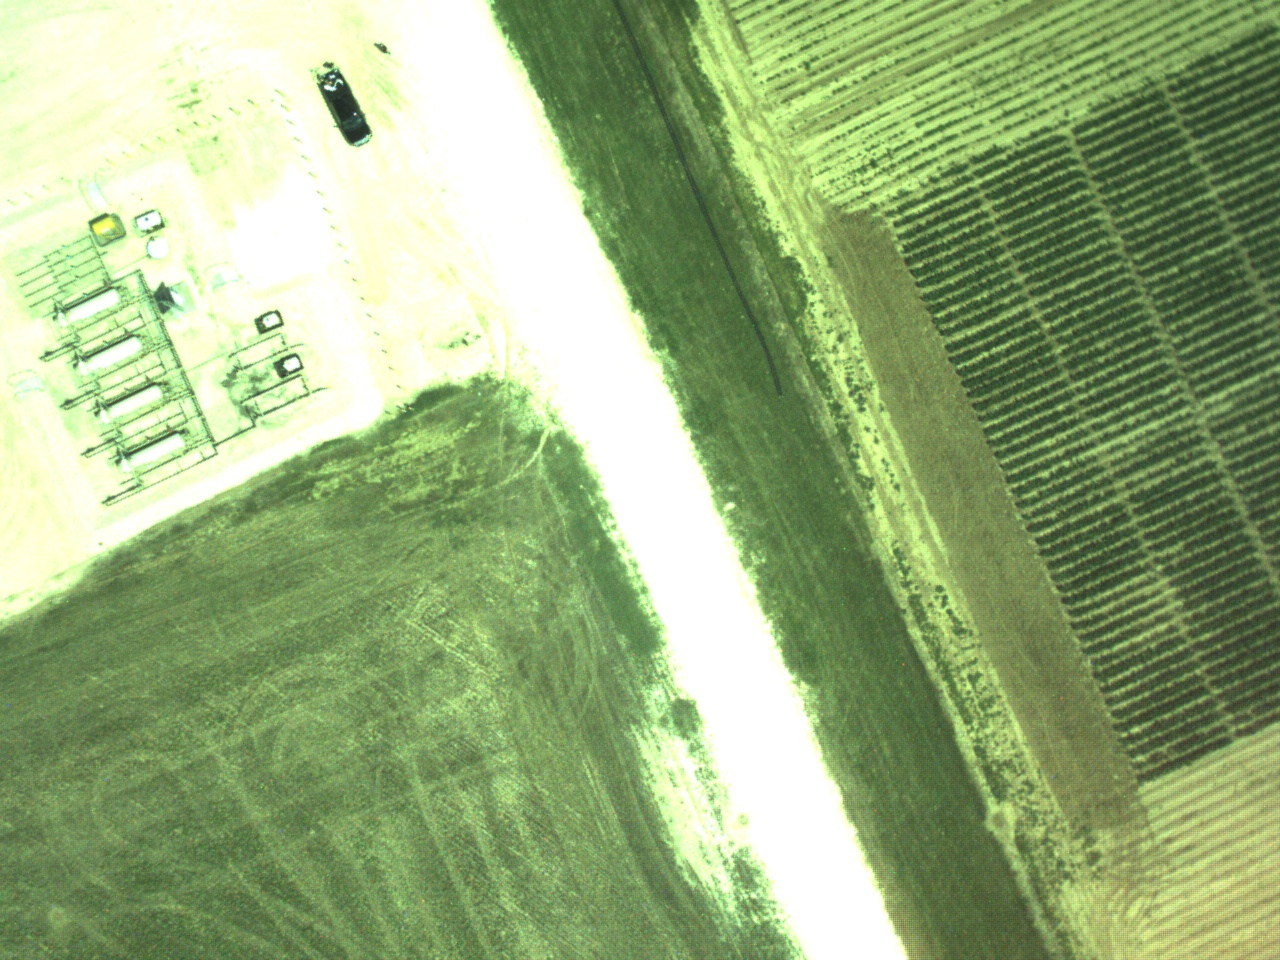
\includegraphics[width = 10cm]{Figures/good2}
\end{centering}
\end{columns}
\end{frame}


\begin{frame} [noframenumbering]
\frametitle{Acceptable Image Stream}
\begin{columns}
\column{0.001\textwidth}
\column{0.999\textwidth}
\begin{centering}
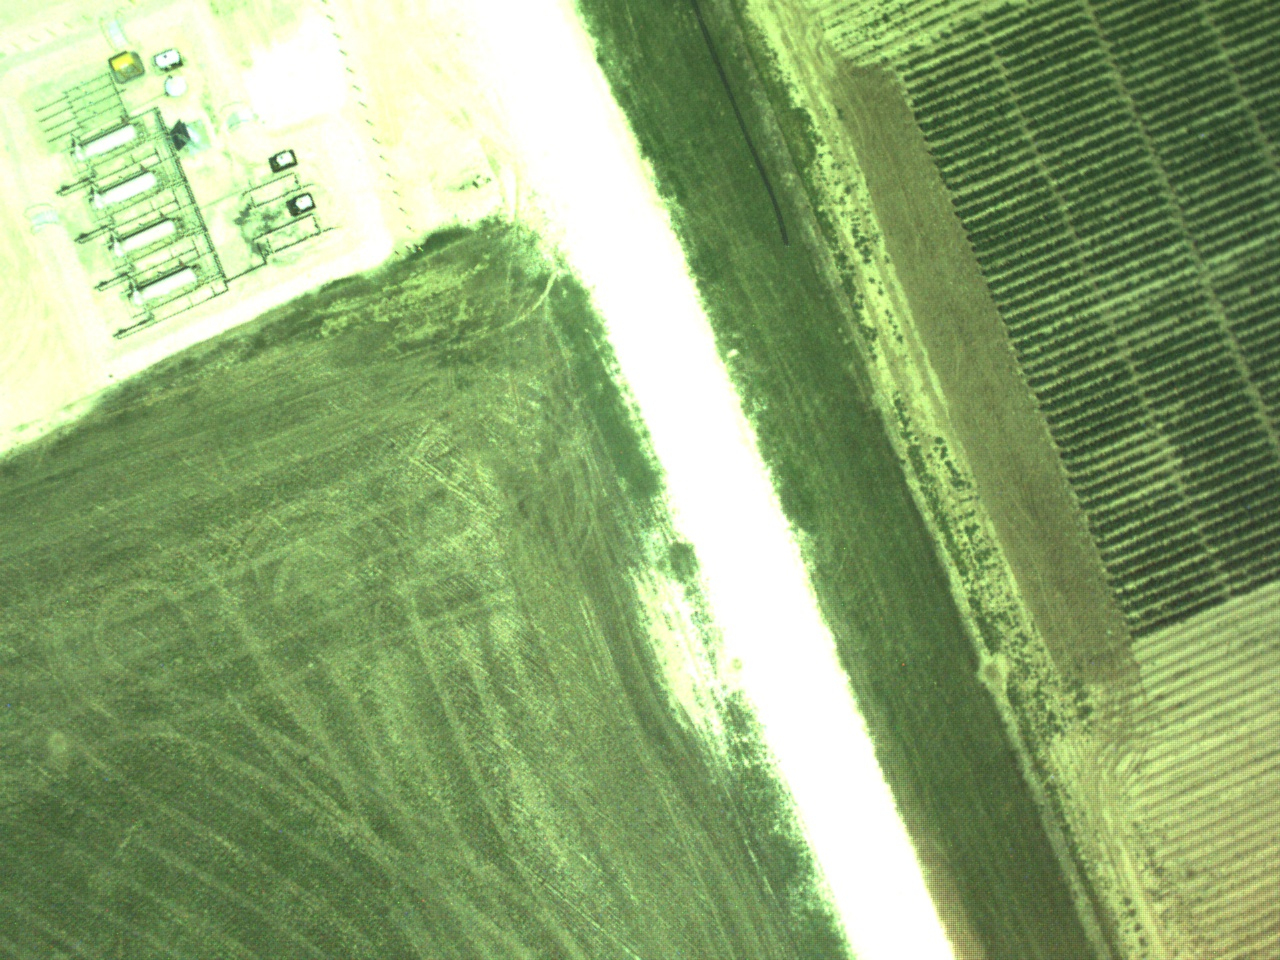
\includegraphics[width = 10cm]{Figures/good3}
\end{centering}
\end{columns}
\end{frame}


\begin{frame} [noframenumbering]
\frametitle{Acceptable Image Stream}
\begin{columns}
\column{0.001\textwidth}
\column{0.999\textwidth}
\begin{centering}
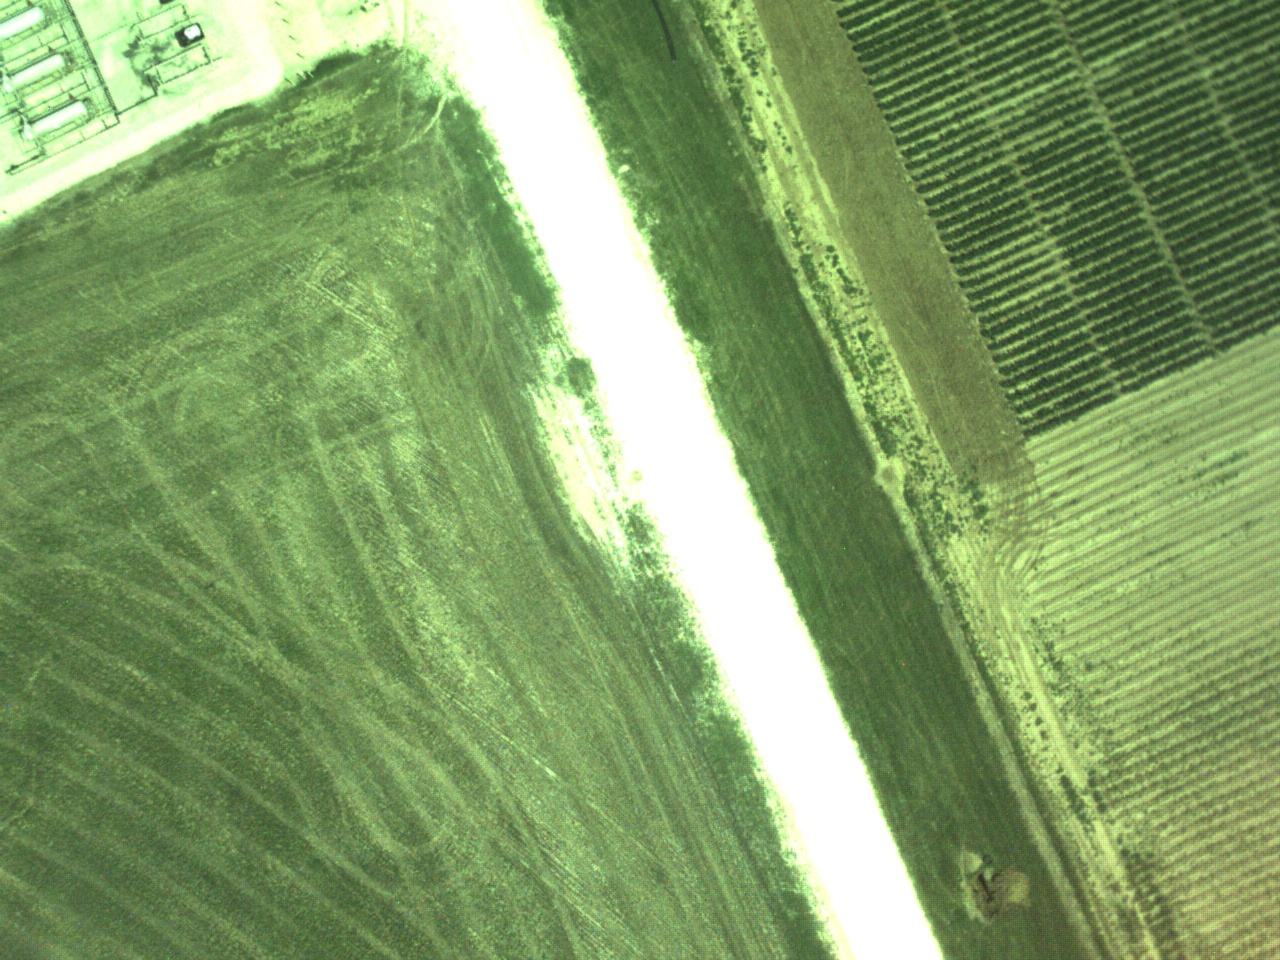
\includegraphics[width = 10cm]{Figures/good4}
\end{centering}
\end{columns}
\end{frame}


\begin{frame} [noframenumbering]
\frametitle{Acceptable Image Stream}
\begin{columns}
\column{0.001\textwidth}
\column{0.999\textwidth}
\begin{centering}
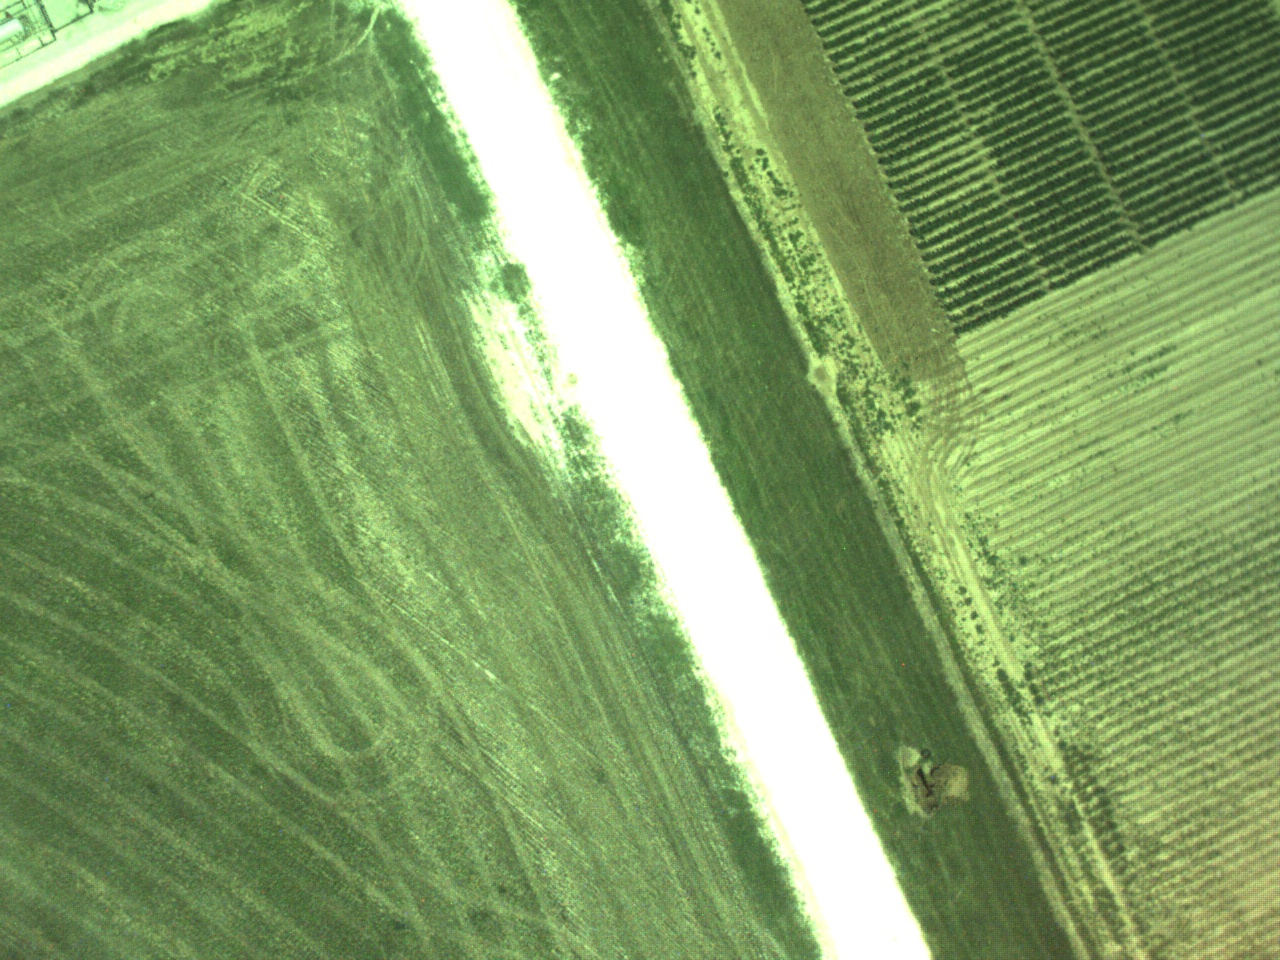
\includegraphics[width = 10cm]{Figures/good5}
\end{centering}
\end{columns}
\end{frame}


\begin{frame}
\frametitle{Anomalous Image Stream}
\begin{columns}
\column{0.001\textwidth}
\column{0.999\textwidth}
\begin{centering}
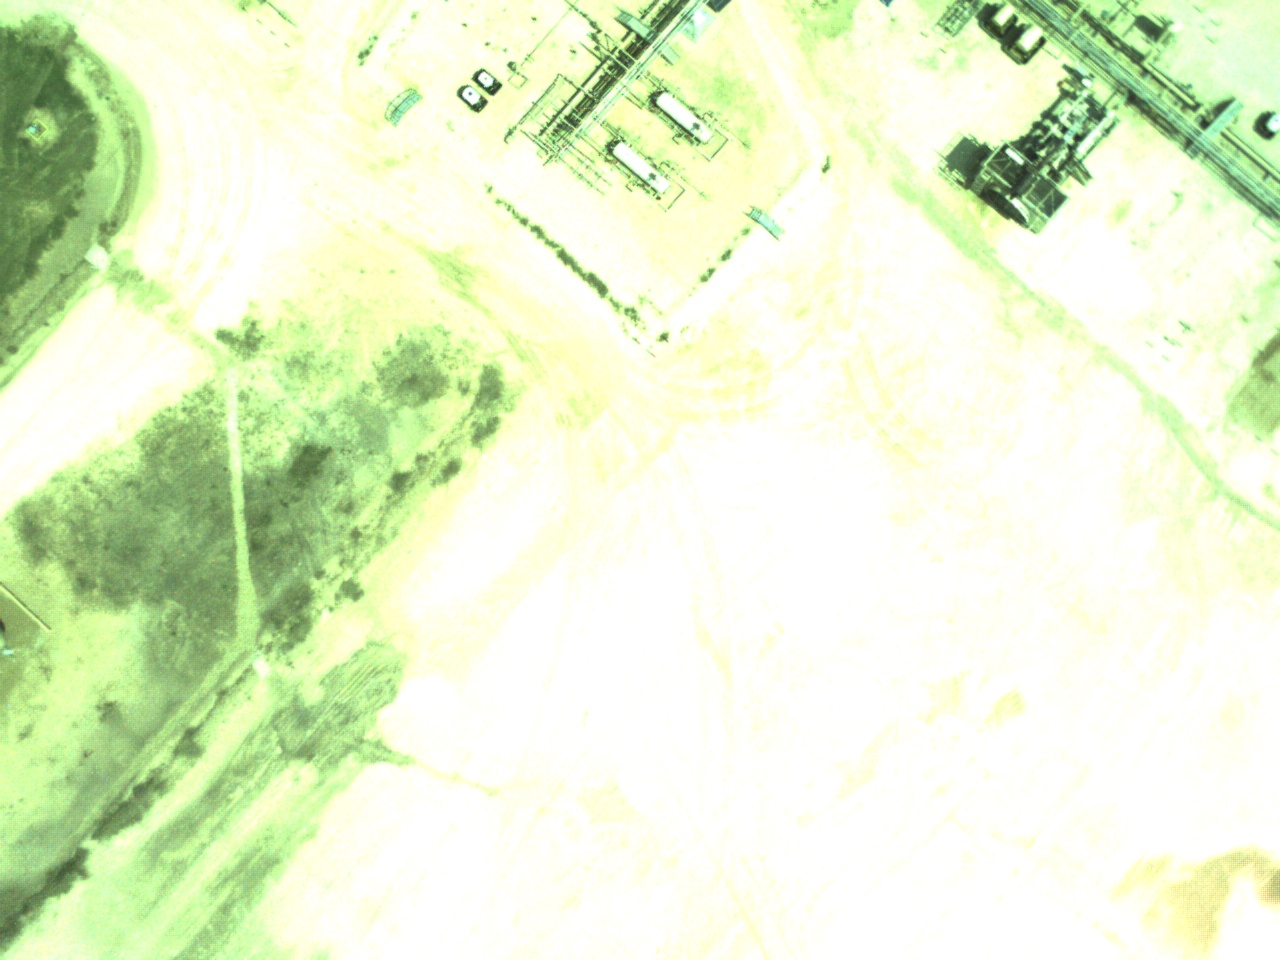
\includegraphics[width = 10cm]{Figures/bad1}
\end{centering}
\end{columns}
\end{frame}


\begin{frame} [noframenumbering]
\frametitle{Anomalous Image Stream}
\begin{columns}
\column{0.001\textwidth}
\column{0.999\textwidth}
\begin{centering}
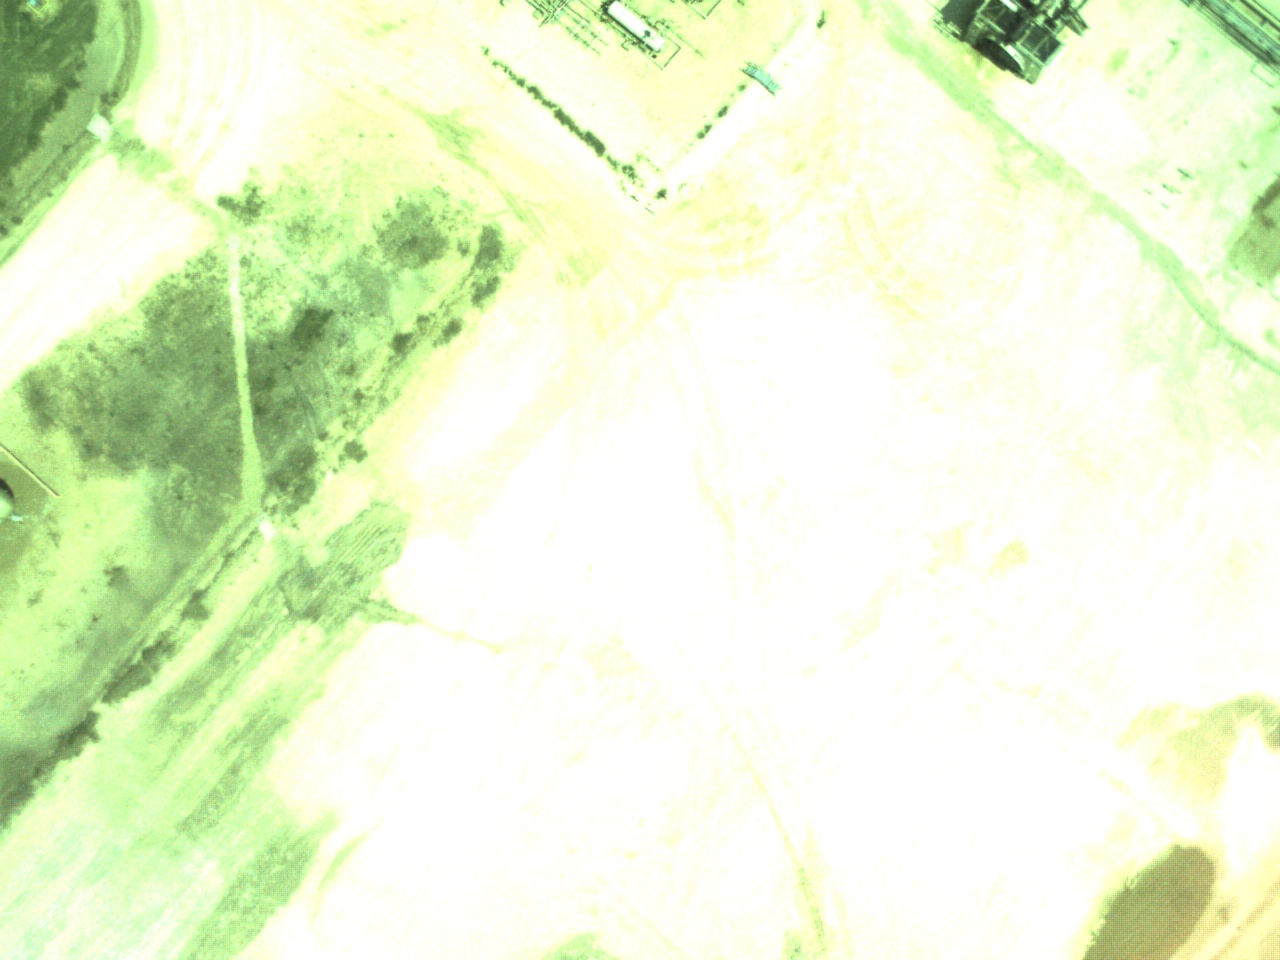
\includegraphics[width = 10cm]{Figures/bad2}
\end{centering}
\end{columns}
\end{frame}


\begin{frame} [noframenumbering]
\frametitle{Anomalous Image Stream}
\begin{columns}
\column{0.001\textwidth}
\column{0.999\textwidth}
\begin{centering}
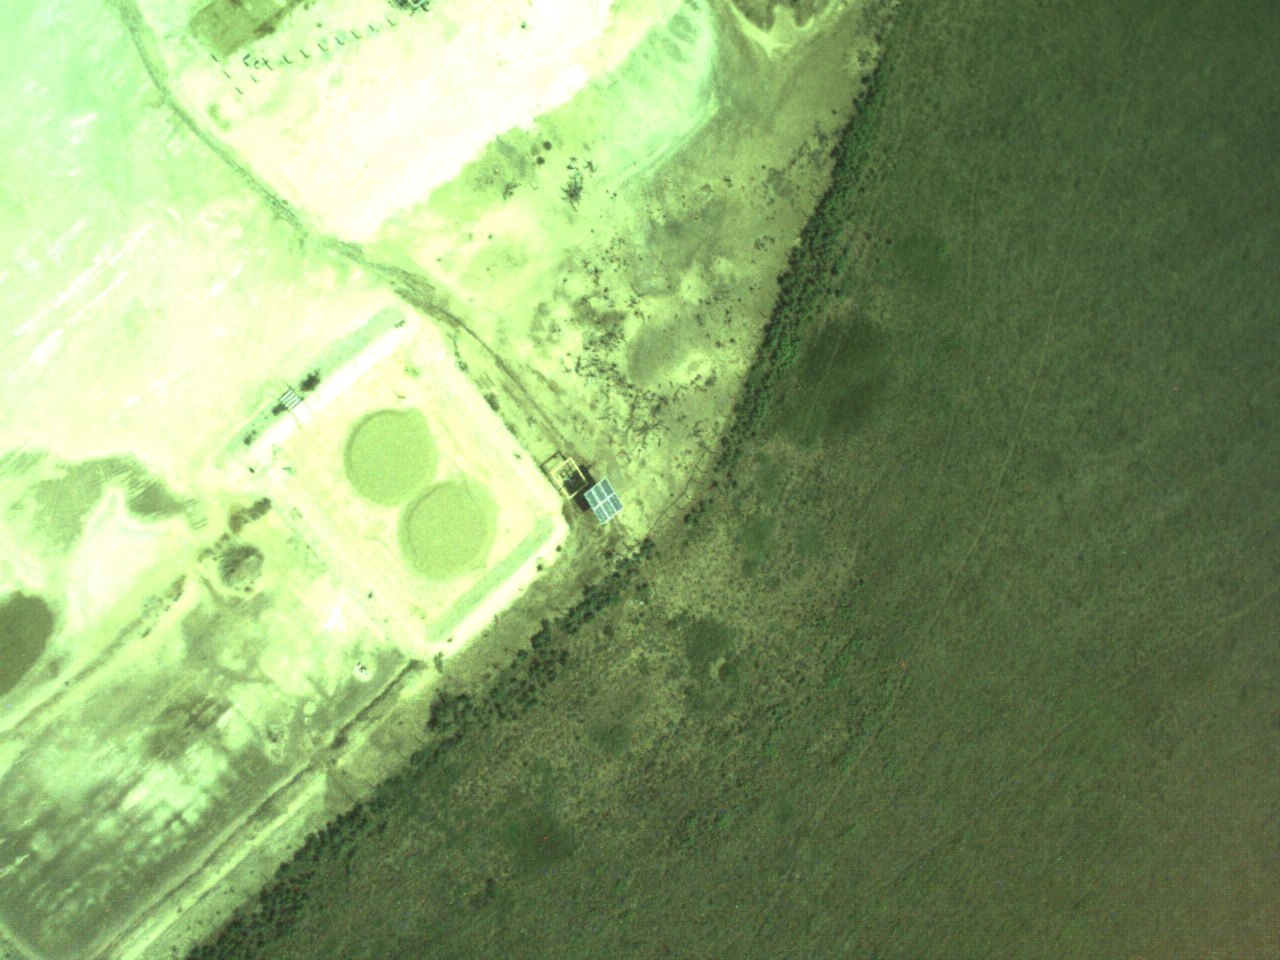
\includegraphics[width = 10cm]{Figures/bad3}
\end{centering}
\end{columns}
\end{frame}


\begin{frame} [noframenumbering]
\frametitle{Anomalous Image Stream}
\begin{columns}
\column{0.001\textwidth}
\column{0.999\textwidth}
\begin{centering}
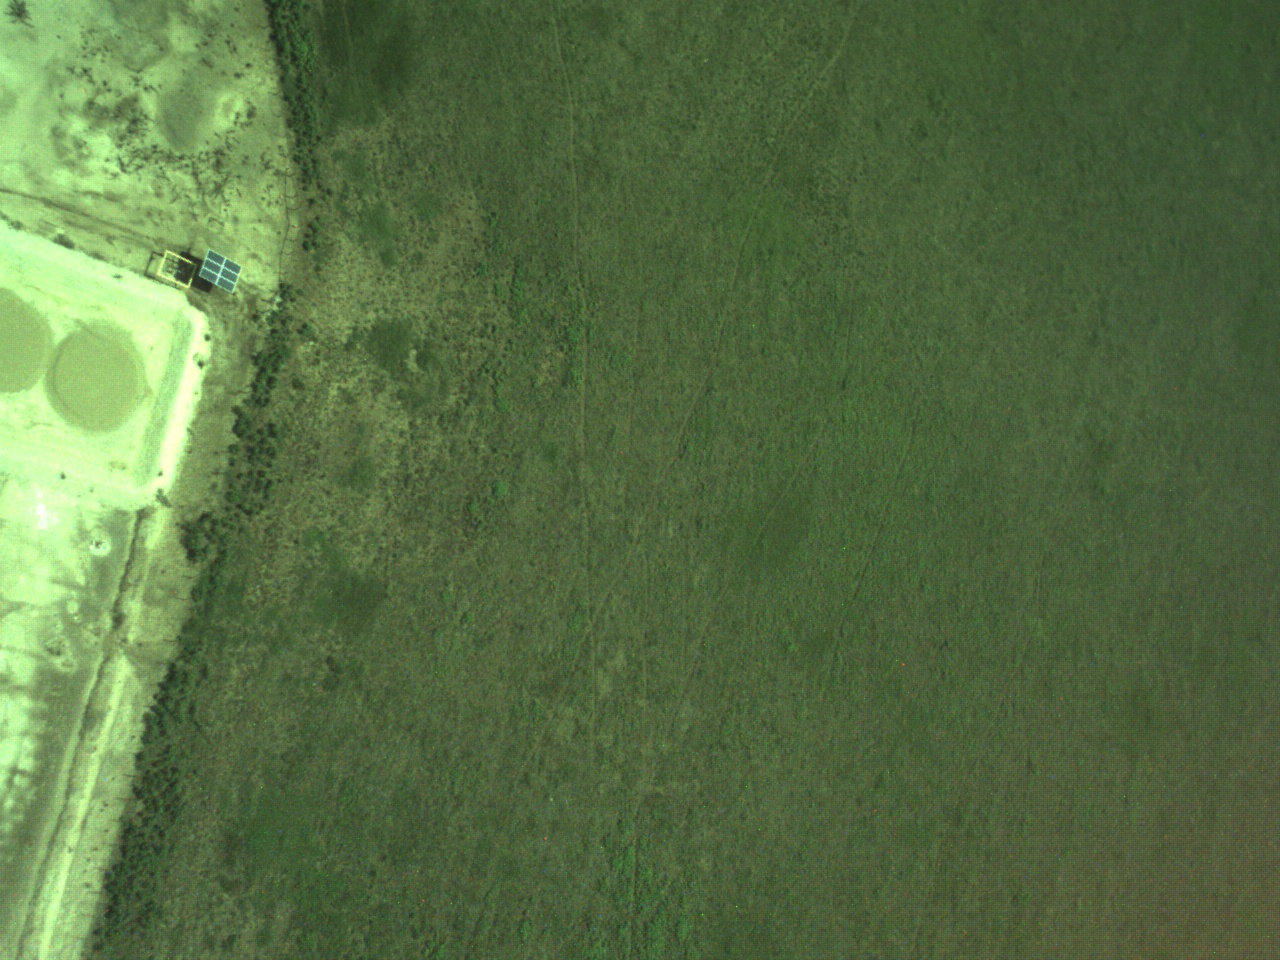
\includegraphics[width = 10cm]{Figures/bad4}
\end{centering}
\end{columns}
\end{frame}


\begin{frame} [noframenumbering]
\frametitle{Anomalous Image Stream}
\begin{columns}
\column{0.001\textwidth}
\column{0.999\textwidth}
\begin{centering}
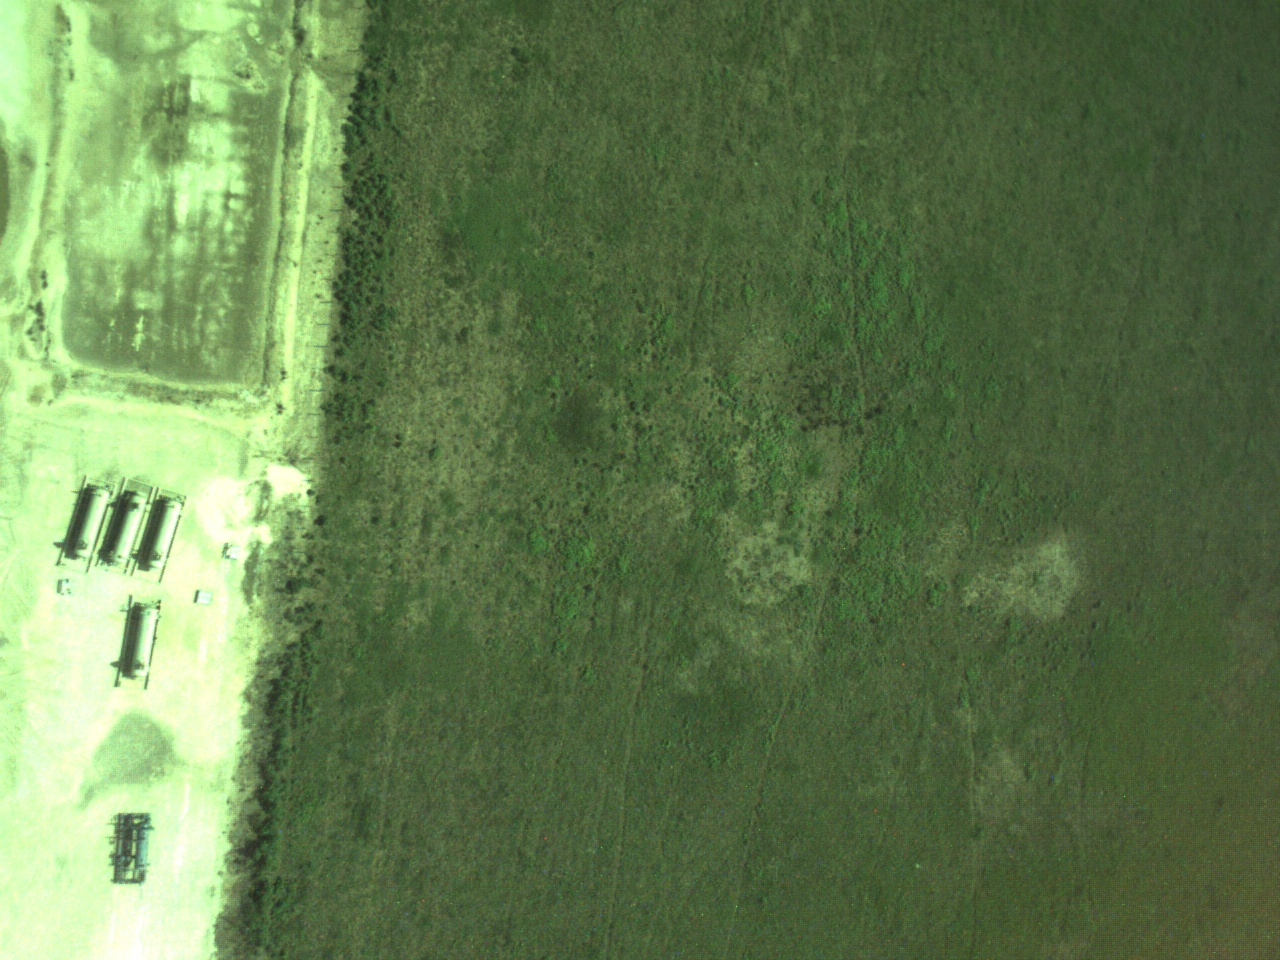
\includegraphics[width = 10cm]{Figures/bad5}
\end{centering}
\end{columns}
\end{frame}


\begin{frame}
\frametitle{Problem Formulation}
\begin{columns}
  \column{0.49\textwidth}
  \begin{itemize}
    \item Traditional methods of determining overlap computationally intensive
    \item Heavily reduce dimensionality by extracting a few features, use machine learning to identify anomalous images
    \item Once a model is trained, extracting features and classifying them requires far less computation
  \end{itemize}
  \column{0.47\textwidth}
  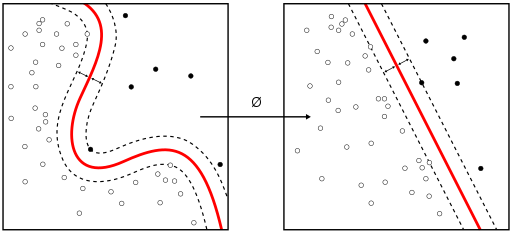
\includegraphics[width = 5cm]{Figures/machinelearning}
\end{columns}
\end{frame}


\begin{frame}
\frametitle{System Model}
\begin{columns}
  \column{0.55\textwidth}
  \scalebox{0.7}{% Define block styles
\tikzstyle{decision} = [diamond, draw, fill=blue!20, 
    text width=4.5em, text badly centered, node distance=3cm, inner sep=0pt]
\tikzstyle{block} = [rectangle, draw, fill=blue!20, 
    text width=4em, text centered, rounded corners, minimum height=4em]
\tikzstyle{wideblock} = [rectangle, draw, fill=blue!20, 
    text width=7em, text centered, rounded corners, minimum height=4em]
\tikzstyle{line} = [draw, -latex']
\tikzstyle{cloud} = [draw, ellipse,fill=red!20, node distance=3cm,
    minimum height=2em]
    
\begin{tikzpicture}[node distance = 2.3cm, auto]
    % Place nodes
    \node [block] (init) {Image stream};
    \node [block, right of=init] (image1) {Shift register};
    \node [block, right of=image1] (image2) {Shift register};
    \node [block, below of=image1] (feature1) {Extract features};
    \node [block, below of=image2] (feature2) {Extract features};
    \node [wideblock, below of=feature2] (mlfeature) {Calculate classification features};
    \node [block, below of=mlfeature] (model) {Learning model};
    \node [wideblock, below of=model] (classification) {Classification};

    % Draw edges
    \path [line] (init) -- (image1);
    \path [line] (image1) -- (image2);
    \path [line] (image1) -- (feature1);
    \path [line] (image2) -- (feature2);
    \path [line] (feature1) -- (mlfeature);
    \path [line] (feature2) -- (mlfeature);
    \path [line] (mlfeature) -- (model);
    \path [line] (model) -- (classification);

\end{tikzpicture}}
  \column{0.43\textwidth}
  \begin{itemize}
    \item Rather than classifying individual images, given our setting we classify image pairs
    \item For each image pair: image features are extracted, classification features are calculated, then passed to the classification model
  \end{itemize}
\end{columns}
\end{frame}


\begin{frame}
\frametitle{Outline}
\begin{itemize}
  \item Introduction
  \item\vspace{0.5cm}Problem Setting
  \item\vspace{0.5cm} \textbf{Image Features}
  \item \vspace{0.5cm}Learning Models
  \item \vspace{0.5cm} Results
  \item \vspace{0.5cm}Conclusions
\end{itemize}
\end{frame}


\begin{frame}
\frametitle{Image Features}
\begin{itemize}
  \item Values, or sets of values, that can be calculated from a digital image
  \item Describe the image in some way
  \begin{itemize}
    \item Smoothness, average brightness, uniformity, number of edges, etc.
  \end{itemize}
  \item Find features which can be extracted quickly, and which should be similar if images share a significant amount of content
  \item Pairs of images: need ways to compare image features between images
\end{itemize}
\end{frame}


\begin{frame}
\frametitle{Pixel Distribution}
\begin{columns}
  \column{0.49\textwidth}
  \begin{itemize}
    \item Discrete distribution of pixel intensity values
    \item 256 bins for integer intensity values between 0 and 255
    \item Large amount of shared content, distributions should be fairly similar
  \end{itemize}
  \column{0.6\textwidth}
  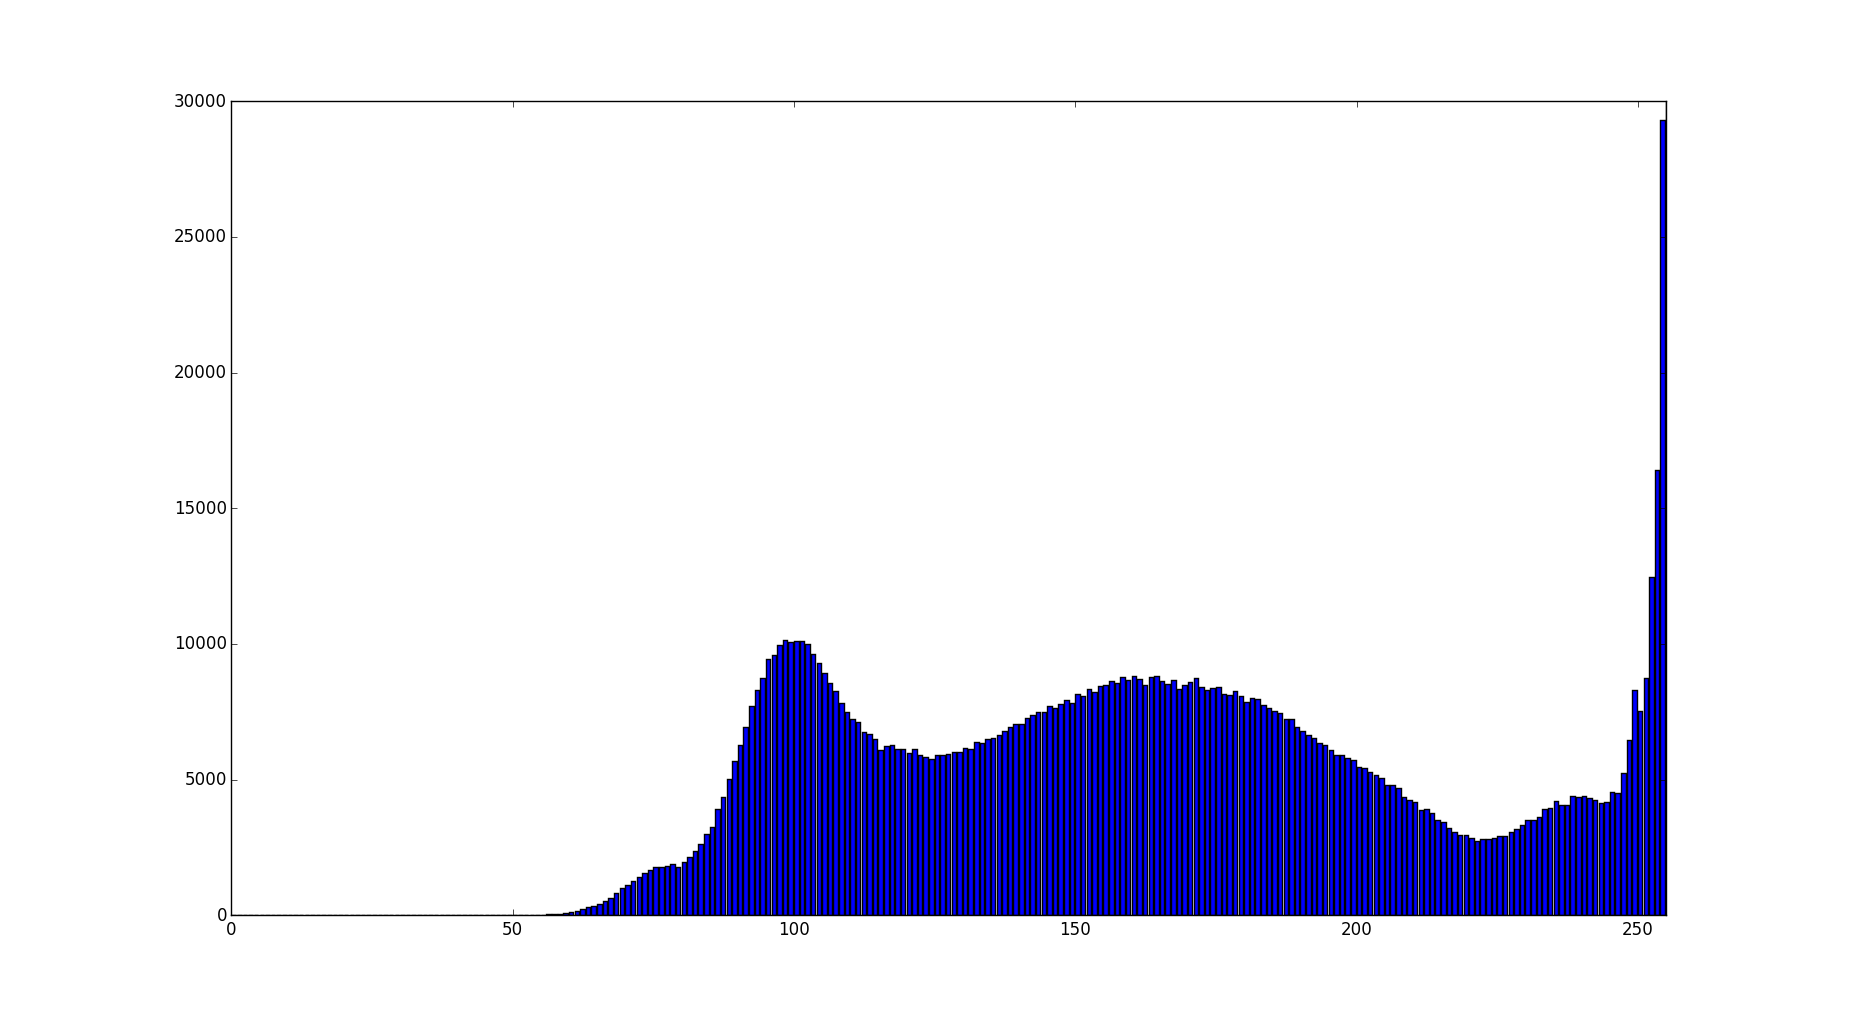
\includegraphics[width = 7cm]{Figures/histogram}
\end{columns}
\end{frame}

\begin{frame}
\frametitle{Pixel Distribution Comparison}
\begin{itemize}
  \item Two discrete distributions $p$ and $q$
  \item Mean squared error
  \begin{itemize}
    \item Common metric to determine a distance between two sets of numbers
    \item $MSE(\mathbf{p}, \mathbf{q}) = \frac{1}{n} \left( \sum_{i=1}^n{(p_i-q_i)^2} \right)$
  \end{itemize}
  \item Bhattacharyya Distance
  \begin{itemize}
    \item Designed for comparing two distributions
    \item $BD(\mathbf{p}, \mathbf{q}) = - \ln \left( \sum_{i=1}^n {\sqrt{p_iq_i}} \right)$
  \end{itemize}
  \item Earth Mover's Distance
  \begin{itemize}
    \item Another metric designed for comparing discrete distributions
    \item Computes the minimum work needed to turn one distribution into another by moving mass between bins
  \end{itemize}
\end{itemize}
\end{frame}


\begin{frame}
\frametitle{MSE Plot}
\begin{columns}
\column{0.001\textwidth}
\column{0.999\textwidth}
\begin{centering}
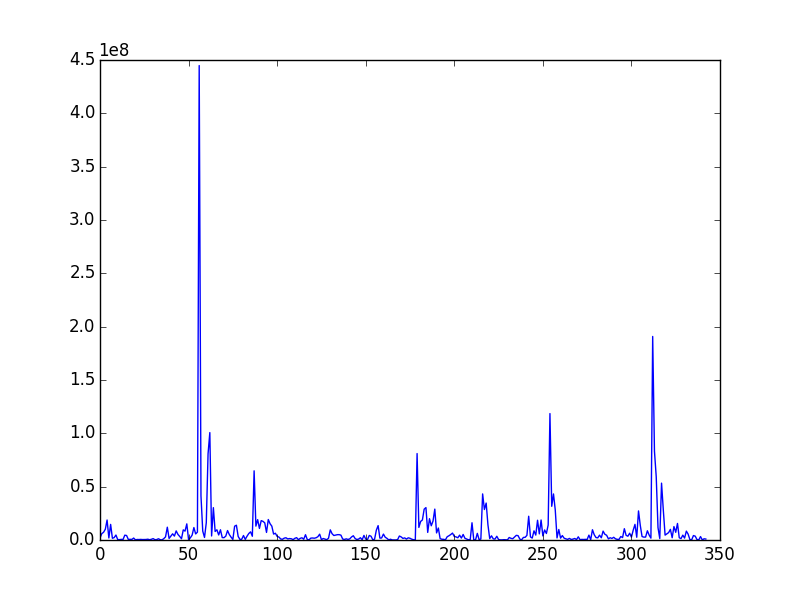
\includegraphics[width = 10cm]{Figures/608MSEplot}
\end{centering}
\end{columns}
\end{frame}


\begin{frame}
\frametitle{Bhattacharyya Distance Plot}
\begin{columns}
\column{0.001\textwidth}
\column{0.999\textwidth}
\begin{centering}
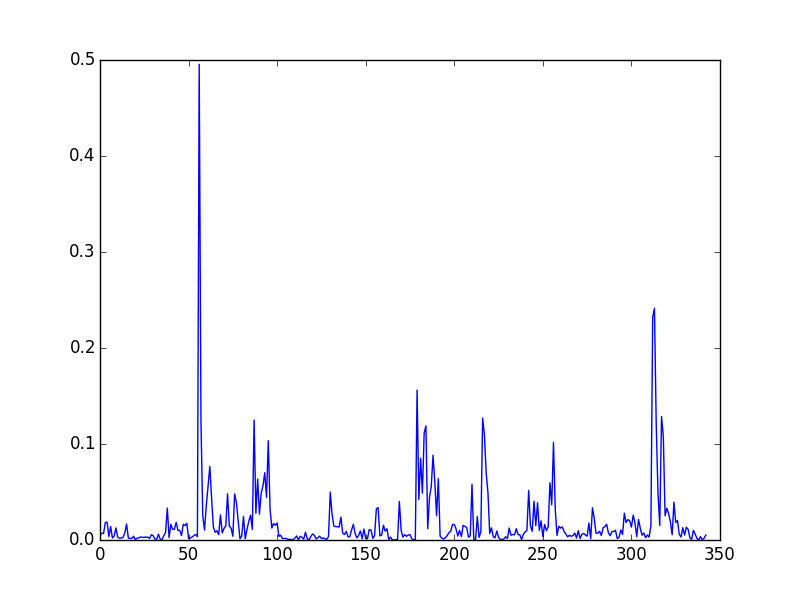
\includegraphics[width = 10cm]{Figures/608BDplot}
\end{centering}
\end{columns}
\end{frame}


\begin{frame}
\frametitle{Earth Mover's Distance Plot}
\begin{columns}
\column{0.001\textwidth}
\column{0.999\textwidth}
\begin{centering}
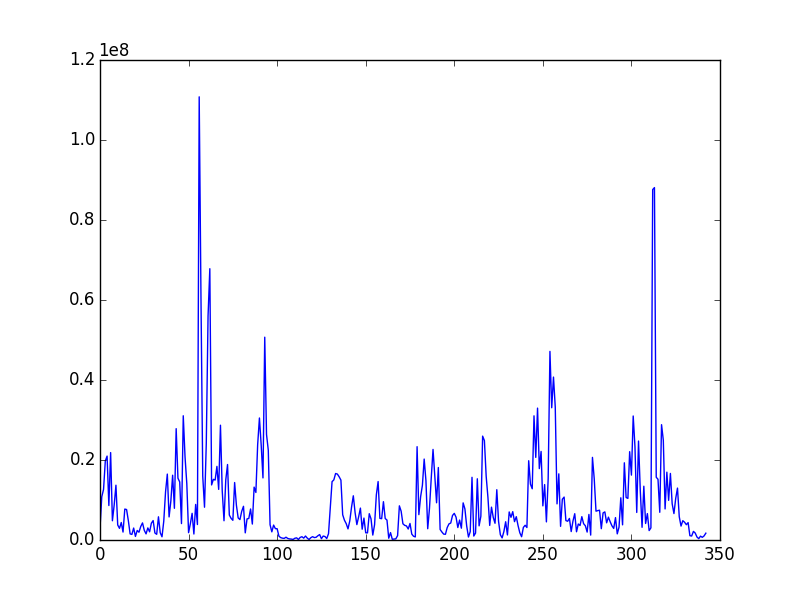
\includegraphics[width = 10cm]{Figures/608EMDplot}
\end{centering}
\end{columns}
\end{frame}



\begin{frame}
\frametitle{BRIEF Descriptors}
\begin{itemize}
  \item Fast computing/matching time and lack of scale-invariance
  \item Select a set number of keypoints using corner, edge, or peak detection
  \item Perform intensity comparisons on patches surrounding keypoints
  \item Results of comparisons form a bitstring, along with the locations of the keypoints forms the descriptor
  \item Descriptors for keypoints can be matched using Hamming distance subject to maximum distance between keypoint locations
\end{itemize}
\end{frame}

\begin{frame}
\frametitle{BRIEF Descriptor Comparison}
\begin{columns}
  \column{0.5\textwidth}
    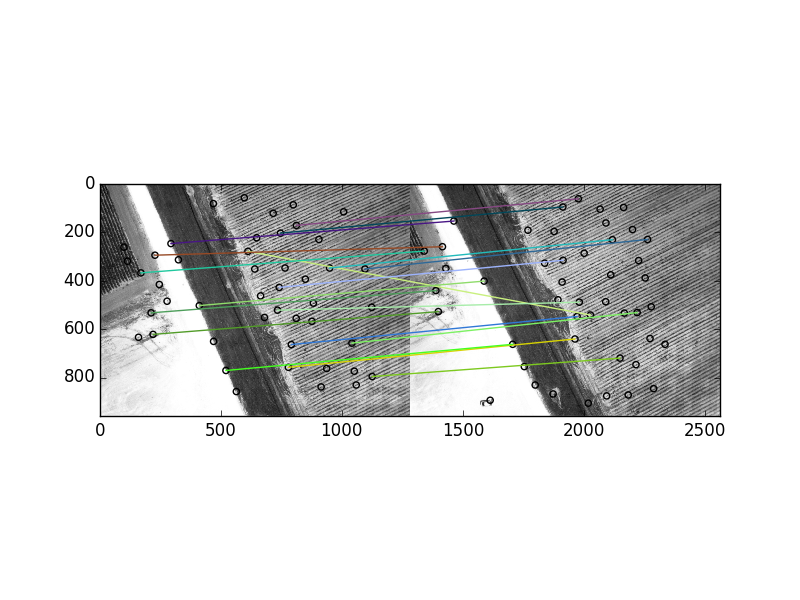
\includegraphics[width = 5cm]{Figures/briefmatchgood}
  \column{0.5\textwidth}
    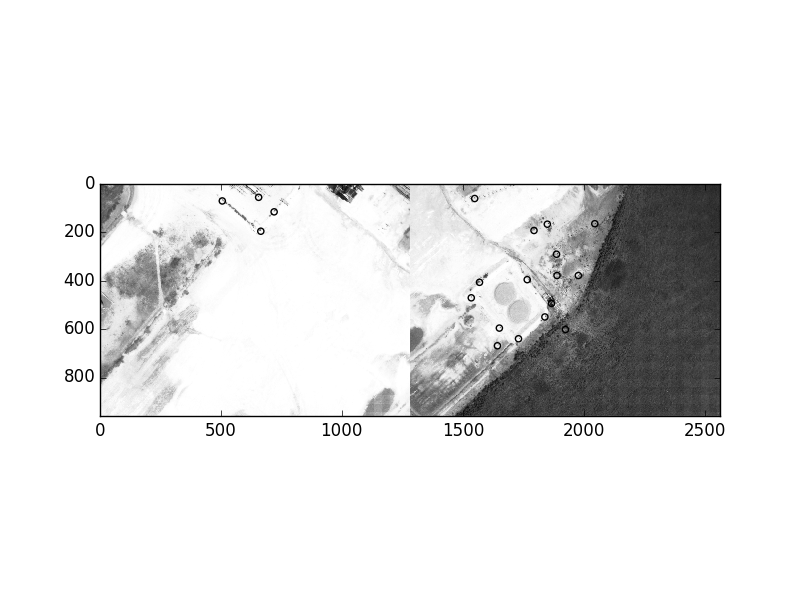
\includegraphics[width = 5cm]{Figures/briefmatchbad}
\end{columns}
  \begin{itemize}
    \item Maximum distance between matched keypoints set to 25\% of image size
    \item Histogram equalization
    \item Number of total matches
    \item Ratio of matches to total keypoints
  \end{itemize}
\end{frame}


\begin{frame}
\frametitle{Blob Detection}
\begin{itemize}
  \item Regions of an image that stand out from the surrounding area (e.g. bright or dark spots)
  \item Similar to keypoints used in BRIEF descriptors, but are a collection of connected pixels
  \item Calculated by convolving image with a Gaussian kernel, then taking the Laplacian
  \begin{itemize}
    \item Strong positive values are the center of a dark blob, strong negative values are the center of a bright blob
  \end{itemize}
  \item Varying sizes of Gaussian kernels to find different sized blobs
\end{itemize}
\end{frame}


\begin{frame}
\frametitle{Blob Comparison}
\begin{columns}
  \column{0.49\textwidth}
  \begin{itemize}
    \item Blob detection results in a list of blob locations and radii
    \item Difference in number of blobs
    \item Using radii, difference in total blob area
  \end{itemize}
  \column{0.47\textwidth}
  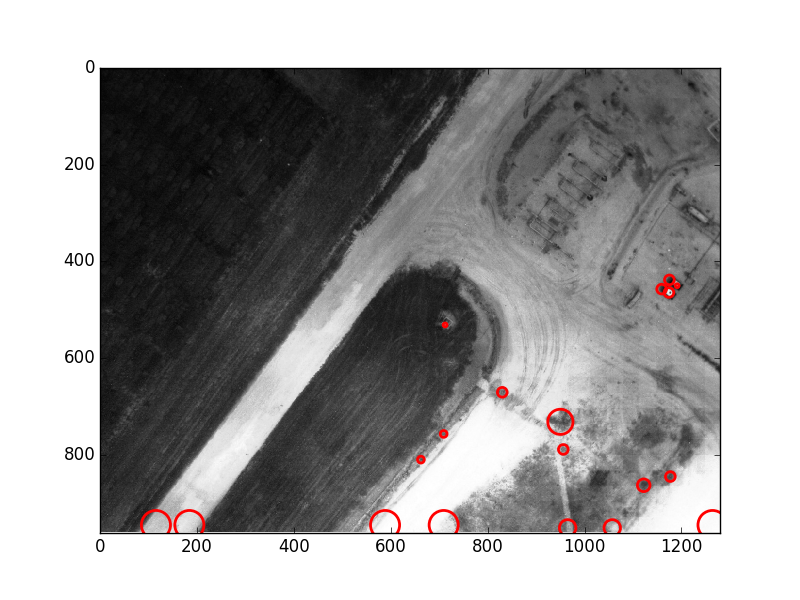
\includegraphics[width = 5cm]{Figures/blobtest}
\end{columns}
\end{frame}


\begin{frame}
\frametitle{Outline}
\begin{itemize}
  \item Introduction
  \item\vspace{0.5cm}Problem Setting
  \item\vspace{0.5cm}Image Features
  \item \vspace{0.5cm} \textbf{Learning Models}
  \item \vspace{0.5cm} Results
  \item \vspace{0.5cm}Conclusions
\end{itemize}
\end{frame}


\begin{frame}
\frametitle{Logistic Regression}
\begin{columns}
  \column{0.49\textwidth}
  \begin{itemize}
    \item Closely related to linear regression
    \item Learns a parameter set $\theta$, s.t. $h_\theta(x) = \frac{1}{1+e^{-\theta^Tx}}$ returns the probability of feature set $x$ belonging to class 1
    \item Gradient descent
  \end{itemize}
  \column{0.47\textwidth}
  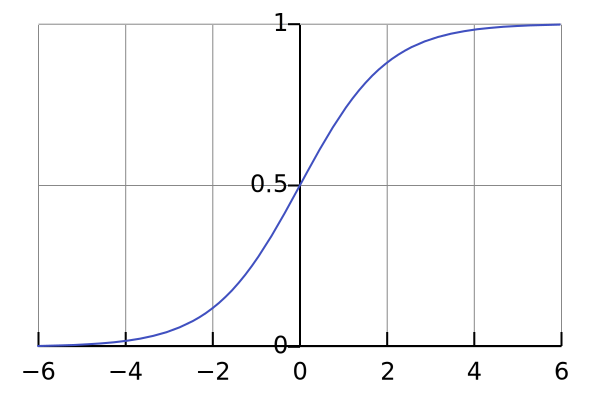
\includegraphics[width = 5cm]{Figures/logit}
\end{columns}
\end{frame}


\begin{frame}
\frametitle{Artificial Neural Network}
\begin{columns}
\column{0.37\textwidth}
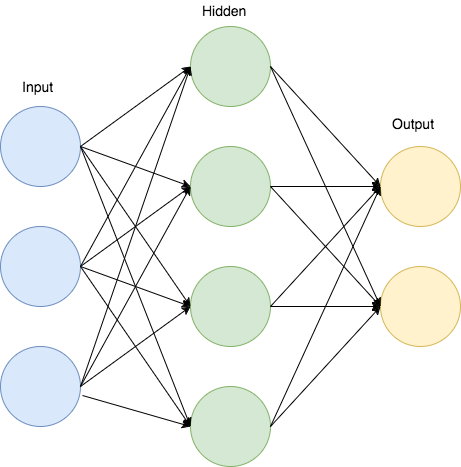
\includegraphics[width = 4.5cm]{Figures/NN}
\column{0.6\textwidth}
\begin{itemize}
  \item Currently very popular for a variety of learning tasks
  \item Inspired by understanding of the human brain
  \item Features input to first layer, propagate through hidden layers according to weights and activation function
  \item Learns connection weights between nodes through backpropagation
  \item Typically requires large amount of training data and tuning
\end{itemize}
\end{columns}
\end{frame}


\begin{frame}
\frametitle{Decision Tree}
\begin{columns}
  \column{0.49\textwidth}
  \begin{itemize}
    \item Generates a tree with the leaf nodes representing classifications
    \item Propagate to child nodes depending on threshold tests 
    \item Learns thresholds based on greedy algorithm - most discriminating split is made at each step
    \item Performs well for simple problems, cannot learn more complex relations between features
  \end{itemize}
  \column{0.45\textwidth}
  \scalebox{0.7}{
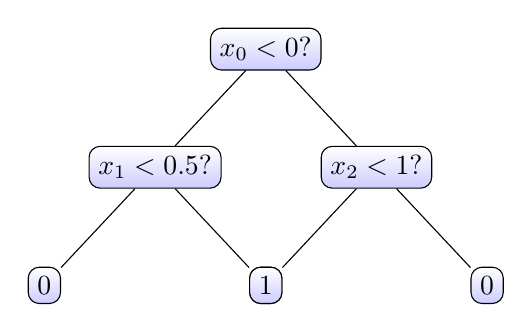
\begin{tikzpicture}[sibling distance=8em,
  every node/.style = {shape=rectangle, rounded corners,
    draw, align=center,
    top color=white, bottom color=blue!20}]]
  \node {$x_0<0?$}
    child { node {$x_1<0.5?$} 
      child { node {$0$}}
      child { node {$1$}}
      }
    child { node {$x_2<1?$} 
      child { node {$1$}}
      child { node {$0$}}
      }

   ;
\end{tikzpicture}}
  \end{columns}
\end{frame}


\begin{frame}
\frametitle{Support Vector Machines}
\begin{columns}
\column{0.47\textwidth}
\includegraphics[width = 5cm]{Figures/svm}
\column{0.49\textwidth}
\begin{itemize}
  \item Maps n-feature vectors to points in n-dimensional space
  \item Learns a hyper-plane that best separates training examples
  \item If linearly separable, learns hard margin with maximum space; if not, learns soft margin that minimizes error
\end{itemize}
\end{columns}
\end{frame}


\begin{frame}
\frametitle{Outline}
\begin{itemize}
  \item Introduction
  \item\vspace{0.5cm}Problem Setting
  \item\vspace{0.5cm}Image Features
  \item \vspace{0.5cm}Learning Models
  \item \vspace{0.5cm} \textbf{Results}
  \item \vspace{0.5cm}Conclusions
\end{itemize}
\end{frame}


\begin{frame}
\frametitle{Implementation}
\begin{columns}
\column{0.49\textwidth}
\begin{itemize}
  \item Python
  \begin{itemize}
    \item NumPy, SciPy, Pandas
  \end{itemize}
  \item Scikit-Image
  \item Scikit-Learn
\end{itemize}
\column{0.47\textwidth}

\includegraphics[width = 5cm]{Figures/scikit}
\end{columns}
\end{frame}


\begin{frame}
\frametitle{Testing Methodology}
\begin{itemize}
  \item Datasets selected and labeled by manually identifying anomalous images
  \begin{itemize}
    \item $\approx$ 5000 images total, $\approx$ 5\% anomalous
  \end{itemize}
  \item Feature vectors generated and associated with label vectors for training and testing of models
  \item Approximately 80\% of data used for training and 20\% used for testing
  \begin{itemize}
    \item Training and testing sets shuffled and retested to obtain average performance
  \end{itemize}
\end{itemize}
\end{frame}


\begin{frame}
\frametitle{Model Tuning}
\begin{itemize}
  \item Depending on the learning model, different methods used to tune hyper-parameters to improve performance
  \item Only 5\% of data in class 1, had to balance data: class weights, resampling
  \item Logistic Regression
  \begin{itemize}
    \item Adjusting learning rate for optimization
  \end{itemize}
  \item Artificial Neural Network
  \begin{itemize}
    \item Adjusting number of hidden layers and number of nodes
  \end{itemize}
  \item Decision Trees
  \begin{itemize}
    \item Depth of tree and number of iterations
  \end{itemize}
  \item SVM
  \begin{itemize}
    \item Since data was not linearly separable, adjusting soft-margin constant
  \end{itemize}
\end{itemize}
\end{frame}


\begin{frame}
\frametitle{Numerical Results}
After repeated training/testing/tuning, the following averaged results were obtained, with detection referring to the percentage of anomalous images detected:
\begin{table}[h!]
  \centering
  \begin{tabular}{|l|l|l|l|}
    \hline
    Algorithm & Detection & False Alarm & Overall  \\ \hline
    Logistic Regression & 0.956 & 0.077 & 0.933  \\ \hline
    Decision Trees & 0.119 & 0.033 & 0.899  \\ \hline
    Neural Network & 0.75 & 0.038 & 0.959  \\ \hline
    SVM & 0.924 & 0.258  & 0.743 \\ \hline
  \end{tabular}
\end{table}
\end{frame}


\begin{frame}
\frametitle{Feature Extraction Times}
Averaged feature extraction times for the features used.
The distribution time includes time to calculate Bhattacharyya distance, other distance metrics amount to a single subtraction or division.
\begin{table}[h!]
  \centering
  \begin{tabular}{|l|l|l|l|}
    \hline
    Distribution & BRIEF & Blobs & Overall  \\ \hline
    0.0473s & 0.244s & 1.06s & 1.351s  \\ \hline

  \end{tabular}
\end{table}
\end{frame}


\begin{frame}
\frametitle{Outline}
\begin{itemize}
  \item Introduction
  \item\vspace{0.5cm}Problem Setting
  \item\vspace{0.5cm}Image Features
  \item \vspace{0.5cm}Learning Models
  \item \vspace{0.5cm}Results
  \item \vspace{0.5cm} \textbf{Conclusions}
\end{itemize}
\end{frame}


\begin{frame}
\frametitle{Interpretation}
\begin{itemize}
  \item Results for logistic regression, SVM, and neural network promising
  \item Feature extraction times reasonable on the order of 1 second, with imaging frequency ranging from 40-80 images per minute
  \item Decision tree provided point of comparison, but performed poorly - too simple
  \item Neural network may perform better with more training data and time
  \item Manually labeled data - borderline cases
  \begin{itemize}
    \item False alarm pseudo-detection
  \end{itemize}
\end{itemize}
\end{frame}

% \begin{frame}
% \frametitle{Challenges}
% \begin{itemize}
%   \item Manually labeling data - borderline cases
%   \item 
% \end{itemize}
% \end{frame}

\begin{frame}
\frametitle{Further Study}
\begin{itemize}
  \item Still a wealth of untested image features
  \item Parallelization of feature extraction
  \item Deeper study into neural networks for this purpose - more data, more time
  \item Actual testing on flight computer
\end{itemize}
\end{frame}


\begin{frame}
\frametitle{ Thank You! }
\begin{itemize}
  \item Questions?
\end{itemize}
\end{frame}


\end{document}

